\section{Оборудование}

\begin{figure}[ht!]
    \centering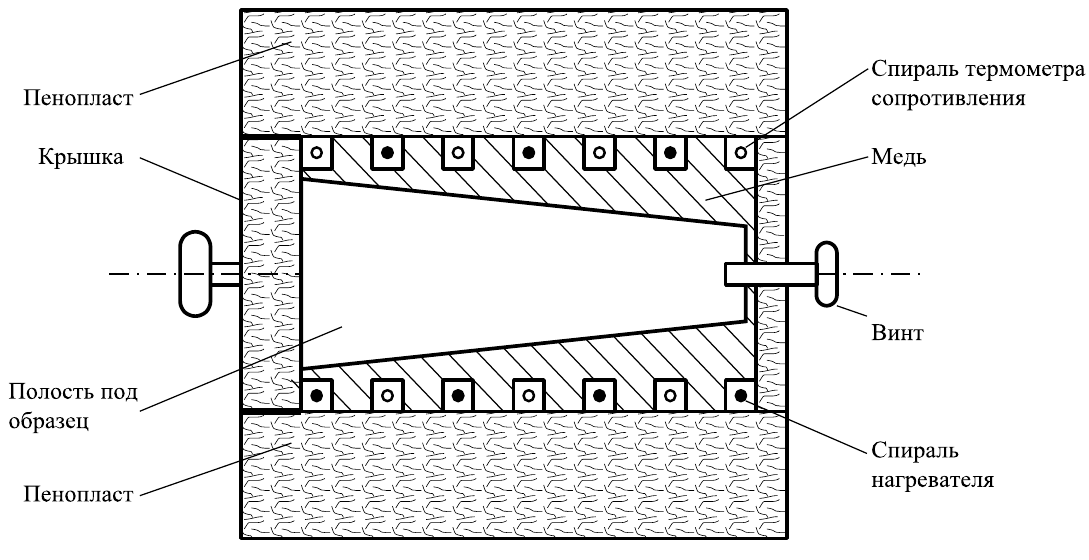
\includegraphics[width=0.8\linewidth]{img/kal.png}
    \caption{Устройство калоиметра}
\end{figure}
\begin{figure}[ht!]
    \centering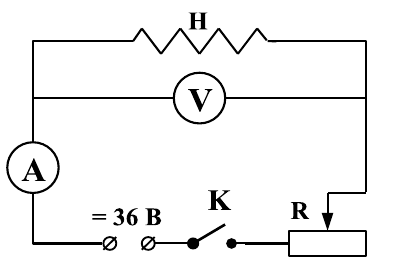
\includegraphics[width=0.8\linewidth]{img/el.png}
    \caption{Схема включения нагревателя}
\end{figure}

Установка состоит из калориметра с пенопластовой изоляцией, помещенного в ящик из
многослойной клеенчатой фанеры. Внутрение стенки калориметра хорошо проводят тепло.
Стенки имеют надёжный тепловой контакт с телом. Они имеют вид усечённых конусов и
плотно прилегают друг к другую. Для выталкивания образца служит винт.

В стенку калориметра смонтированы нагреватель и термометр сопротивления. Схема
включения нагревателя изображена на рисунке 2.

Мощность определяется по амперметру и вольтметру, сопротивление~--- по омметру.

Измеряемые данные:
\begin{enumerate}
    \item $R_\text{heat}(t)$~--- зависимость термометра сопротивления от времени нагревания (с включенным нагревателем)
    \item $R_\text{cool}(t)$~--- зависимость термометра сопротивления при охлаждении (с выключенным нагревателем)
    \item $R_\text{K}(t)$~--- зависимость комнатной температуры
\end{enumerate}

Все кривые записываются с шагом по оси времени $\Delta t = 1\,\text{с}$

Сопротивление термометра сопротивления меняется по закону
\[R=R_{273}\left(1+\alpha \left(T-273\right)\right)\]
$R$~--- сопротивление при температуре $T$, $R_{273}$~--- сопротивление при $273\,\text{K}$.

\[T=273+\frac{R_\text{T}}{\alpha R_\text{K}}\left(1+\alpha\left(T_{\text{K}}-273\right)\right)-\frac{1}{\alpha}\]

$\alpha=4{,}28\cdot 10^{-3}\,\text{K}^{-1}$

\[CdT_\text{cool}=-\lambda\left(T_\text{cool}-T_\text{K}\right)dt\]
\[T_\text{cool}=\left(T-T_\text{K}\right)e^{-\frac{\lambda}{C}t}+T_\text{K}\]

Тангенс угла наклона этой прямой в координатах $\left(\ln\frac{T_\text{cool}-T_\text{K}}{T-T_\text{K}};t\right)$
равен $\frac{\lambda}{C}$

\[CdT_\text{heat}=Pdt-\lambda\left(T_\text{heat}-T_\text{K}\right)dt\]
\[\frac{CdT_\text{heat}}{P-\lambda\left(T_\text{heat}-T\text{K}\right)}=dt\]
\[T_\text{heat}=\frac{P}{\lambda}\left(1-e^{-\frac{\lambda}{C}t}\right)+T_\text{K}\]
Отсюда можно найти $\lambda$, а из $\lambda$ и $\frac{\lambda}{C}$~--- $C$.

При больших колебаниях температуры этот метод дает большую погрешность и лучше
использовать дифференциальный метод.

\[C=\frac{P}{\left(\frac{dT_\text{heat}}{dt}\right)_{T=T_\text{K}}}\]

$A=\left(\frac{dT}{dt}\right)_\text{heat}$, $B=\left(\frac{dT}{dt}\right)_\text{cool}$,
$T_\text{heat}=T_\text{cool}=T$
\[\lambda=\frac{P}{\left(T-T_{\text{K}_2}\right)\left(1-\frac{A}{B}\right)+T_\text{K2}-T_\text{K1}}\]
\[C=\frac{P}{A-B+A\frac{T_\text{K1}-T_\text{K2}}{T-T_\text{K1}}}\]
